\documentclass{article}
\usepackage[margin=.5in]{geometry}
\usepackage{graphicx, dblfloatfix}
\usepackage{amsmath, amssymb, amsfonts, mathrsfs, mathtools, physics}
\usepackage[english]{babel}
\usepackage[autostyle, english = american]{csquotes}
\usepackage[normalem]{ulem}
\usepackage[title,titletoc,toc]{appendix}
\usepackage{pgfplotstable}
\usepackage{array, booktabs, colortbl, caption}
\usepackage{braket}
\MakeOuterQuote{"}

\newcommand{\redchi}{$\tilde{\chi}^2\,$}
\renewcommand{\vec}[1]{\mathbf{#1}}

\title{Optical Absorption Edge in Semiconductors}
\author{Alejandro Legarda}

\begin{document}
\raggedright
\maketitle

\begin{abstract}
.
\end{abstract}


\tableofcontents
\newpage

\section{Theory}

Atoms have discrete electron energy levels, but when atoms are brought together to form a solid, the electron orbitals overlap and interact to form wider energy bands. Such bands represent a continuum of allowed energies and adjacent bands may either overlap or be separated by a band gap depending on the structure and atoms that make up the material.

\hspace{.25cm}

\begin{figure}[!htb]
	\centering
	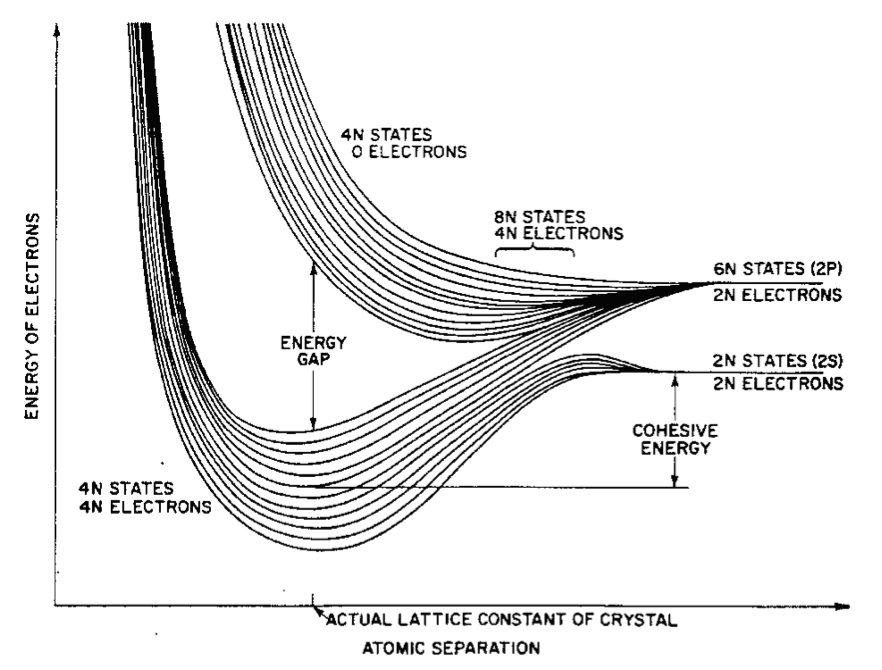
\includegraphics[scale=.5]{plots/fig_1.png}
 	\label{bands}
	\caption{An example of energy levels broadening into energy bands and energy gaps. N atoms, each with 4 electrons, move from distinct s and p energy states at large separation (far right of the plot) to two nearly continuous bands at smaller separation.}
\end{figure}

\hspace{.25cm}

Electrons organize themselves within bands of a solid analogously to the discrete energy levels of a single atom. The innermost (core) electrons are bound tightly to the nuclei and fill the lowest energy bands. The valence electrons contribute to chemical bonds. The next higher energy band is the conduction band. Electrons in the conduction band are no longer bound to the nucleus and can thus move freely in the material. Electrons can be excited from the valence band into the conduction band by the absorption of energy from incident photons or from phonons. When an electron is excited from the valence to the conduction band, it leaves behind a hole of +1 charge in the valence band. An excited electron can return to the valence band by means of recombination with the hole.

\hspace{.25cm}

In semiconductors, the valence and conduction bands are separated by a small band gap, typically 0.1-1 eV. At room temperature, some electrons are thermally excited to the conduction band, but most remain in the valence band. The smallness of the band gap, however, means electrons can be promoted from the valence to conduction bands by absorption of photons with energies near the visible range.

\begin{thebibliography}{10}

	\bibitem{labmanual}
		University of Chicago Department of Physics. "Optical Absorption Edge in Semiconductors"\\
		https://wiki.uchicago.edu/display/P211manuals/Optical+Absorption+Edge+in+Semiconductors. (Accessed May, 2016)

	\bibitem{taylor}
		Taylor, John. \emph{An Introduction to Error Analysis}. Sausalito: University Science Books, 1997.
		
\end{thebibliography}
